\section{Overview of state databases} \label{Overview of state databases}

\subsection{Databases implementing Andmejälgija}

\begin{itemize}
    \item{Digiregistratuur}
    \item{Elamislubade ja töölubade register}
    \item{Kinnistusraamat}
    \item{Kutseregister}
    \item{Maksukohustuslaste register}
    
    \item{Politsei taktikalise juhtimise andmekogu}
    \item{Põllumajandusloomade register}
    \item{Põllumajandustoetuste ja põllumassiivide register}
    \item{Rahvastikuregister}
    \item{Retseptikeskus}
    \item{Sotsiaalkaitse infosusteem}
    \item{Sotsiaalteenuste ja toetuste register}
    \item{Tööinspektsiooni tooelu infosusteem}
    \item{Töötuskindlustuse andmekogu}
\end{itemize}
POLIS Information System, while in the list of the Andmejälgija view on Eesti.ee, actually doesn't show any entries even if they should be there.

\subsection{Databases providing other form of data access tracking}
\begin{itemize}
    \item{E-toimik}: provides it's own web-view for displaying requests made about you.
    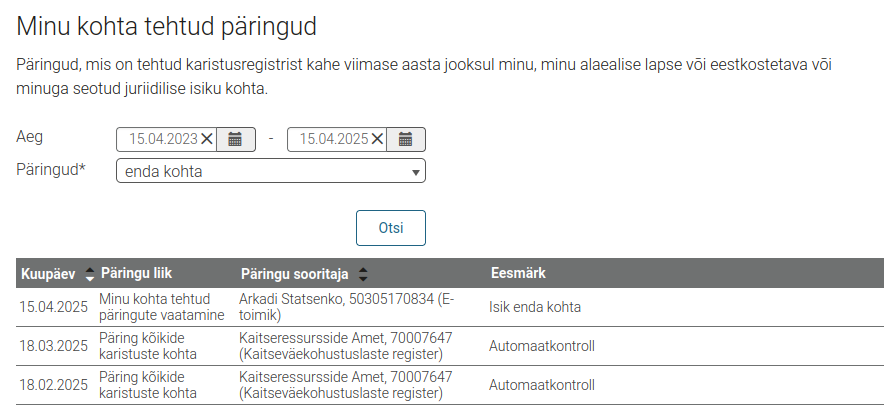
\includegraphics[width=450px]{english/figures/e-toimik.png}
\end{itemize}




\subsection{Databases not providing any kind of data access tracking}
\begin{itemize}
    \item{Schengen Information System}
    \item{Piirikontrolli andmekogu (PIKO)}
    \item{Infosusteem POLIS}
\end{itemize}
